\documentclass[11pt,a4paper,sans]{report}
%%%%%%%%%%%%%%%%%%%%%%%%%%%%%%%%%HEADER FROM ADRIAN SATIN, modified by william fabre %%%%%%%%%%%%%%%%%%%%%%%%%%%%%%%%%%%%%%
\usepackage[utf8]{inputenc} 
\usepackage{graphicx} % support the \includegraphics command and options
\usepackage[frenchb]{babel}
\usepackage{tikz}
\usepackage{circuitikz}
\usetikzlibrary{circuits}
\graphicspath{{images/}}% chemin vers les images
\usepackage[parfill]{parskip} % Activate to begin paragraphs with an empty line rather than an indent
%%% PACKAGES
\usepackage{hyperref} % Gestion Hyperliens/url
% https://en.wikibooks.org/wiki/LaTeX/Hyperlinks
\usepackage{eurosym}
\usepackage{fancyhdr}
\usepackage{color}
\usepackage{svg}
% YOLO NICE CODE EXEMPLE merci axel
\usepackage{minted}
\usepackage{paralist} % very flexible & customisable lists (eg. enumerate/itemize, etc.)
\usepackage{verbatim} % adds environment for commenting out blocks of text & for better verbatim
\usepackage{subfig} % make it possible to include more than one captioned figure/table in a single float
\usepackage{graphicx}
\usepackage{fancyhdr}
\usepackage{multicol}
\usepackage{listings}
\usepackage{listings}
\usepackage{amsmath,amsfonts,amsthm,amssymb}
\usepackage{pdfpages}
\usepackage{comment}
\usepackage{caption}
\definecolor{violet-logo}{RGB}{23,63,28}
%%% HEADERS & FOOTERS
\usepackage{fancyhdr} % This should be set AFTER setting up the page geometry
\pagestyle{plain} % options: empty , plain , fancy
\renewcommand{\headrulewidth}{1pt} % customise the layout...
\lfoot{}\cfoot{\thepage}\rfoot{}
%%% SECTION TITLE APPEARANCE
\usepackage{sectsty}
\allsectionsfont{\sffamily\mdseries\upshape} % (See the fntguide.pdf for font help)
% (This matches ConTeXt defaults)
%%% ToC (table of contents) APPEARANCE
\usepackage[nottoc,notlof,notlot]{tocbibind} % Put the bibliography in the ToC
\usepackage[titles,subfigure]{tocloft} % Alter the style of the Table of Contents
\renewcommand{\cftsecfont}{\rmfamily\mdseries\upshape}
\renewcommand{\cftsecpagefont}{\rmfamily\mdseries\upshape} % No bold!
\usepackage{geometry} % to change the page dimensions
\geometry{left=2cm, right=2cm, bottom= 1cm}
\geometry{a4paper} % or letterpaper (US) or a5paper or....
\geometry{a4paper} % or letterpaper (US) or a5paper or....
\pagestyle{fancyplain}
\fancyhead{}
%%% END Article customizations

%nice chapter
\usepackage{titlesec}
\titleformat{\chapter}[display]
{\normalfont\bfseries}{}{0pt}{\Large}
\titlespacing*{\chapter}{0pt}{-50pt}{40pt}

% nice section
\makeatletter
\def\@seccntformat#1{%
	\expandafter\ifx\csname c@#1\endcsname\c@section\else
\csname the#1\endcsname\quad
  \fi}
\makeatother

\usepackage{array,multirow,makecell}
\setcellgapes{1pt}
\makegapedcells
\newcommand{\HRule}{\rule{\linewidth}{0.5mm}} % Defines a new command for the horizontal lines, change thickness here
\fancyhf{} % sets both header and footer to nothing
\renewcommand{\headrulewidth}{0pt}
\addtolength{\topmargin}{-60pt}

%bibtex
\bibliographystyle{plain}

% defining my own style for code
\usepackage{xcolor}
\definecolor{codegreen}{rgb}{0,0.6,0}
\definecolor{codegray}{rgb}{0.5,0.5,0.5}
\definecolor{codepurple}{rgb}{0.58,0,0.82}
\definecolor{backcolour}{rgb}{0.95,0.95,0.92}

\lstdefinestyle{mystyle}{
	basicstyle=\fontsize{7}{11}\ttfamily %proper font size
	backgroundcolor=\color{backcolour},   
	commentstyle=\color{codegreen},
	keywordstyle=\color{magenta},
	numberstyle=\tiny\color{codegray},
	stringstyle=\color{codepurple},
	basicstyle=\ttfamily\footnotesize,
	breakatwhitespace=false,         
	breaklines=true,                 
	captionpos=b,                    
	keepspaces=true,                 
	numbers=left,                    
	numbersep=5pt,                  
	showspaces=false,                
	showstringspaces=false,
	showtabs=false,                  
	tabsize=2
}

\lstset{style=mystyle}


\begin{document}
\begin{titlepage}

	\center % Center everything on the page

	%----------------------------------------------------------------------------------------
	%	HEADING SECTIONS
	%----------------------------------------------------------------------------------------

	\textsc{\LARGE Université Pierre et Marie Curie}\\[1.5cm] % Name of your university/college
	\textsc{\Large projet MANET}\\[0.5cm] % Major heading such as course name

	%----------------------------------------------------------------------------------------
	%	TITLE SECTION
	%----------------------------------------------------------------------------------------
	\vfill
	\HRule \\[0.4cm]
	{ \huge \bfseries Compte-rendu : Projet ARA 2019–2020, Mobile Ad hoc NETworks }\\[0.4cm] 
	\HRule \\[1.5cm]
	\vfill
	%----------------------------------------------------------------------------------------
	%	AUTHOR SECTION
	%----------------------------------------------------------------------------------------

	\begin{minipage}{0.4\textwidth}
		\begin{flushleft} \large
			\emph{Auteurs:}\\
			% Ordre alphabetique sur les noms
			\textsc{Maria Popova, William Fabre} 
		\end{flushleft}
	\end{minipage}
	~
	\begin{minipage}{0.4\textwidth}
		\begin{flushright} \large
			\emph{Professeur:} \\
			Monsieur \textsc{Lejeune},\textsc{Favier}
		\end{flushright}
	\end{minipage}\\[2cm]

	%----------------------------------------------------------------------------------------
	%	DATE SECTION
	%----------------------------------------------------------------------------------------

	{\large Année 2019-2020}\\[2cm] % Date, change the \today to a set date if you want to be precise

\end{titlepage}

\newpage
\tableofcontents
\vspace*{3cm}
\begingroup\let\clearpage\relax

	\newpage
	\chapter{Introduction}

	%multilinecomments
	\begin{comment}
		TODO intro du projet, nos remarques. + Explication du fichier de config accompagnées d’un fichier texte "Readme"
		indiquant comment compiler le projet et lancer les différentes simulations (votre projet doit pouvoir se compiler/lancer en dehors d’Eclipse) Votre rapport, au format pdf, concis, dans lequel vous devez répondre aux questions posées dans le sujet.
	\end{comment}

	% TODO quotation work use the biblio.bib to add references.
	TODOCHANGEHEREtest1234\cite{greenwade93}

	\newpage
	\chapter{Préparation du projet et installation}
	% TODO tutoriel d'installation
	\newpage
	\chapter{Exercice 1 – Implémentation d’un MANET dans Peer-Sim}

	\section{Question 1}
	\textit{En analysant le code de la classe PositionProtocolImpl, donnez l’algorithme général de déplacement d’un nœud. Il ne vous est pas demandé de copier/coller le code dans cette question.}
	\par Le but de cet algorithme est de deplacer un noeud dans l'espace de deux dimenssions en direction d'une position choisi en fonction de la strategie de deplacement.  L'algorithme de deplacement du noeud fonctionne comme suit :
	\par Si le noeud ne bouge pas alors il est mis en mouvement. C'est a dire q'on lui affecte une vitesse \texttt{vi} aleatoire bornee par un \texttt{MinSpeed} et un \texttt{MaxSpeed}. Puis on lui choisi une desination qui est de type Position (element qui possede deux coordonnes). Il faut maintenant calculer la distance en metres entre le point de depart, qui est la position du Node et la position d'arrivee, que nous appellerons destination ; Grace a la formule suivante :
	\begin{gather}
		Soit \quad  (dest, cur) \in Position^2, \\
		distance = (dest.x - cur.x)^2 + (dest.y - cur.y)^2 
	\end{gather}
	\par C'est la distance total pour arriver a destination. Maintenant il nous faut calculer la distance totale parcourable en une unite de temps. Elle est egale a la vitesse dans la metrique du systeme, c'est a dire, la vitesse \texttt{vi} en metres par secondes qu'il faut diviser par mille pour avoir des metre par millisecondes.
	\begin{gather}
		Soit  \quad  (vi) \in Vitesse \quad (m*s^{-1}), \\
		distance\_to\_next= vi / 1000
	\end{gather}
	\par Si la distance totale est inferieur a la distance parcourable en une unite de temps il faut alors calculer une nouvelle Position intermediaire et donc un x et un y:

	\begin{gather}
		Soit  \quad  (next_x,next_y) \in long^2 \\
		Soit  \quad  (\theta_{1}, \theta_{2}) \in degree^2 \\
		next\_x =  (distance\_to\_next * \dfrac{(dest.x - cur.x)}{((dest.x - cur.x)^2 + (dest.y - cur.y)^2)}) + cur.x \\
		\Longleftrightarrow \\
		next\_x =  (distance\_to\_next * \sin{\theta_{1}}) + cur.x \\
		\\
		\\
		next\_y =  (distance\_to\_next * \dfrac{(dest.y - cur.y)}{((dest.x - cur.x)^2 + (dest.y - cur.y)^2)}) + cur.y \\
		\Longleftrightarrow \\
		next\_y =  (distance\_to\_next * \cos(\theta_{2})) + cur.x \\
	\end{gather}

	Sinon, si la distance total est egale ou inferieur a la distance parcourable en une unite de temps, alors on affete les coordonnes de la position destination a notre Node.

	% TODO expliquer mieux.
	On vient verifier si la position a change, pour affecter une pause; Sinon on incremente le temps du simulateur d'une unite de temps.

	\section{Question 2}
	\textit{Testez le simulateur en prenant la stratégie FullRandom comme SPI et SD. Le contrôleur graphique sera déclenché toutes les unités de temps, son timeslow pourra être environ de 0.0002. Le seul protocole à renseigner pour ce contrôleur est le PositionProtocol de la simulation, les autres sont pour l’instant optionnels et sans objet.  Normalement vous devez voir graphiquement des points verts se déplacer sur l’écran.  N’oubliez pas d’amorcer les instances de PositionProtocol via un module d’initialisation. Vous répondrez à cette question en donnant le contenu de votre fichier de configuration.}
	% TODO Ajouter des commentaires explicatifs (beaucoup)
	\mylisting[basicstyle=\tiny,frame=rlbt,language=Java]{../src/ara/config} %with frame

	\newpage
	\section{Question 3}
	\textit{Codez une classe implémentant l’interface Emitter. Testez de nouveau avec le moniteur graphique et assurez-vous que les portées sont représentées (cercle en bleu).}
	% TODO Ajouter des commentaires explicatifs a la classe mais essayer de ne pas depasser une page
	\mylisting[basicstyle=\tiny,frame=rlbt,language=Java, firstline=14, lastline=124]{../src/ara/manet/communication/EmitterProtocolImpl.java}
	%\lstinputlisting[language=Java]{\communication}


	\section{Question 4}
	% Peut etre expliquer les difficultes?

	\section{Question 5}
	\par\textit{Testez votre code, et remarquez sur le moniteur graphique l’apparition d’un lien graphique lorsque deux nœuds deviennent voisins.}
	\begin{figure}[h]
		\centering
		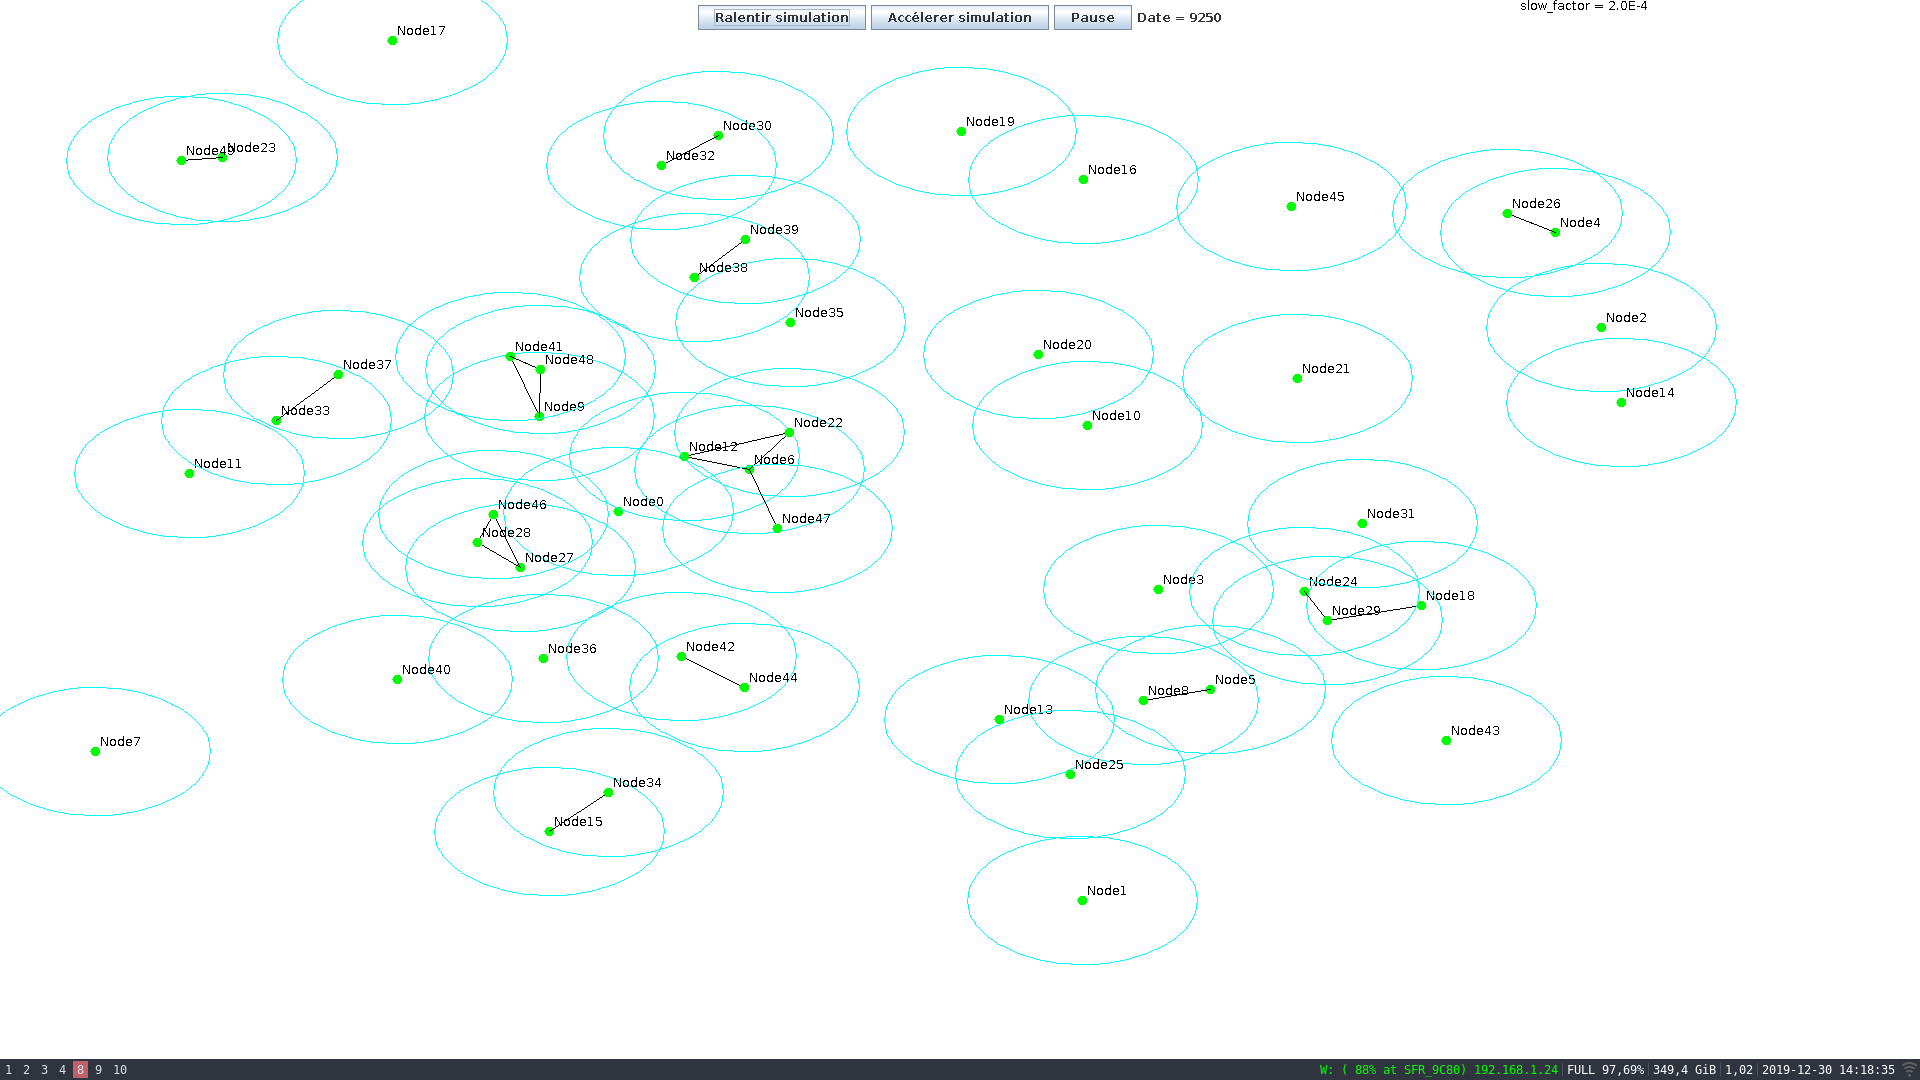
\includegraphics[width=\textwidth, frame]{question5_links}
		\caption{Representation de l'apparition de lien lors de la simulation}
		\label{fig:mesh1}
	\end{figure}


	% TODO ecrire un commentaire intelligible ici on peut voir comment referencer une figure
	% on peut aussi comment referencer directement la page d'une figure
	\par As you can see in the figure \ref{fig:mesh1}, the 
	function grows near 0. Also, in the page \pageref{fig:mesh1} 
	is the same example.

	\section{Question 6}
	\textit{En analysant les codes des classes gérant le positionnement des nœuds qui font appel à un tirage aléatoire, on peut remarquer qu’ils utilisent un objet Random qui leur est dédié (attribut my\_random initialisé au random de la classe PositioningConfiguration).  Quelle en est la raison ?}

	Le but de nos simulations est d'evaluer un ensemble d'algorithme avec differents types de placement, deplacements de nodes. la reproductibilite de ces simulations est importante pour des soucis de debug ou de l'analyse. Maitriser tres exactement la seed de randomization est un point cle pour avoir des algorithmes avec des placements aleatoires mais maitrises. On peut voir que la classe \texttt{PositioningConfiguration} recuperer \texttt{PAR\_SEED\_POSITIONING} depuis le fichier de configuration.

	\section{Question 7}
	\textit{Prenez connaissance des différentes stratégies et pour chacune expliquez ce qu’elle fait.}
	Pour chacune les strategies de placement de noeuds dans l'espace il existe deux types de placement : Un placement dit initial et un deplacement qui sont represente par deux fonctions :
	\texttt{getInitialPosition} et \texttt{getNextDestination}. Les strategies implementent ces fonctions si elles implementent leur interfaces : \texttt{InitialPositionStrategy} et \texttt{NextDestinationStrategy} ceci sera precise dans le titre des sections suivantes.

	\subsection*{Strategie 1 : ConnectedRandom (InitialPositionStrategy, NextDestinationStrategy)}
	\subsubsection{\texttt{getInitialPosition} et \texttt{getNextDestination}}
	\par Le schema suivant s'applique pour definir une position initial ou trouver une nouvelle position a un noeud.

	\begin{figure}[H]
		\centering
		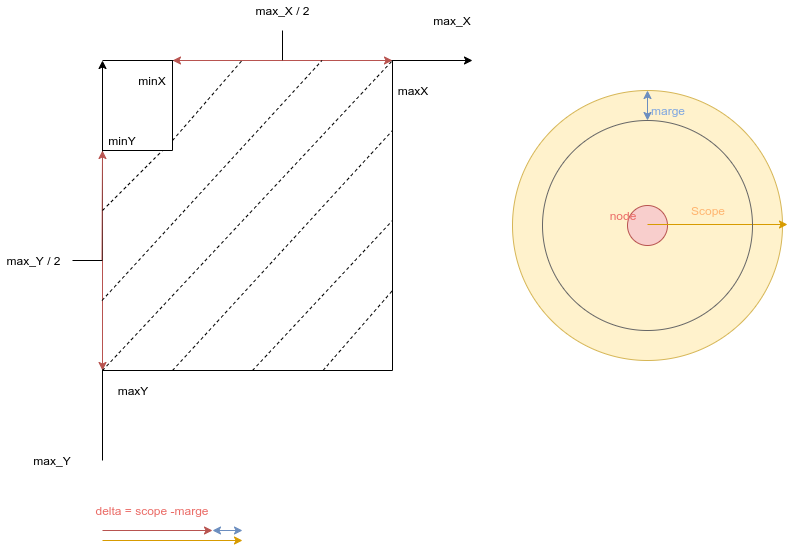
\includegraphics[width=0.9\textwidth, frame]{StrategieConnectedRandom}
		\caption{Representation du calcule pour le placement connected Random}
		\label{fig:mesh1}
	\end{figure}


	\par Les elements de la figure \ref{fig:mesh1} sont :
	\begin{itemize}
		\item A gauche, la grille de placement des noeuds avec \texttt{max\_X} et \texttt{max\_Y} qui sont des parametres du systeme. On peut aussi voir \texttt{max\_X / 2} et \texttt{max\_Y / 2}. Pour finir, \texttt{maxX, maxY, minX, minY} correspondent aux nouveaux min et max calcules par la fonction en additionnant ou soustrayant delta visible graphiquement. La zone hachuree correspond a l'ensemble des coordonnees possible pour une position randomizee.
		\item A droite, On peut observer le scope d'un noeud et un parametre de marge de l'algorithme Connected Random.
		\item En bas on peut observer graphiquement la taille de \textt{scope-marge}
	\end{itemize}

	La figure ci dessus\pageref{fig:mesh1} represente l'implementation pour les fonctions \texttt{getInitialPosition} et \texttt{getNextDestination}, il existe un argument de fonction speed qui n'est pas utilise malgre le fait que l'interface \texttt{NextDestinationStrategy} explique : "Retourne une nouvelle de destination du neoud host en fonction de la vitesse speed".

	\newpage
	\subsection*{Strategie 2 : FullRandom (InitialPositionStrategy, NextDestinationStrategy)}

	\subsubsection{\texttt{getInitialPosition}}
	\par La strategie pour la position initiale est de creer en une table associative a partir de tous les noeuds du reseau et grace a la fonction \texttt{Network.get(i)} ("Returns node with the given index. Note that the same node will normally have a different index in different times. le ieme dans la liste des noeuds", ce qui signifie un ajout de randomization) affecter a chaque node le resultat de la fonction Destination decrite ci-apres.

	\subsubsection{\texttt{getNextDestination}}
	\par La strategie de choix de la destination suivante consiste a affecter une nouvelle position \textt{nextX} et \textt{nexty} tel que :
	\begin{gather}
		position = (my\_random.nextDouble() * maxX, \quad my\_random.nextDouble() * maxY)
	\end{gather}


	\subsection*{Strategie 3 : InitialPositionConnectedRing (InitialPositionStrategy)}
	\subsubsection{\texttt{getInitialPosition}}
	Le but de cette fonction est de calculer la position des points en fonction d'un centre pour les placer autour de celui-ci. Elle utilise : \texttt{centre.getNewPositionWith} qui "Calcul une nouvelle position à partir d'un module et d'un angle depuis la position courante".
	Explicitons les calcules, nous reutiliserons les variables \texttt{maxX, maxY, scope maxX/2 et maxY/2}, nous ajoutons une variable centre qui est definie par les coordonnes \texttt{maxX/2,MaxY/2}, la taille du reseau, appelee \texttt{size} et une variable rayon qui nous aidera a placer les points autour du centre.
	\begin{gather}
		Soit \quad rayon \in Entier, \\
		rayon = min(size*(scope/8), maxY / 2.5) \\
		\\
		exemple \quad : \\ 
		size = 10 \quad scope = 32 \quad maxY = 500 \\
		rayon = min(10*4, 500/2.5) \\
		rayon = min(40, 200) = 40
	\end{gather}
	Le calcule du rayon differe si les noeuds sont paires ou impaires. voici la fin du calcule s'ils sont paire :
	\begin{gather}
		Soit \quad rayon \in Entier, \\
		Soit \quad numero\_de\_node \in Entier paire, \\
		rayon = rayon - (scope/2) \\
		\\
		exemple \quad : \\ 
		rayon = 40 - (32/2) = -210
	\end{gather}
	Il faut maintenant un \texttt{delta\_angle} qui servira au calcule de la position cournte de la fonction \texttt{center.getNewPositionWith},
	\begin{gather}
		Soit \quad delta\_angle \in Entier, \\
		delta\_angle = \dfrac{2 * \pi}{size} \\ 
		\\
		exemple \quad : \\ 
		size = 10 \\
		delta\_angle = \dfrac{2 * \pi}{10} = 0.6283 \quad(approx)\\ 
	\end{gather}

	\par l'appelle a la fonction  :
	\begin{lstlisting}
		centre.getNewPositionWith(rayon, delta_angle * host.getID())
	\end{lstlisting}
	\par placera donc les noeuds de 0 a 9 ainsi :
	\begin{figure}[H]
		\centering
		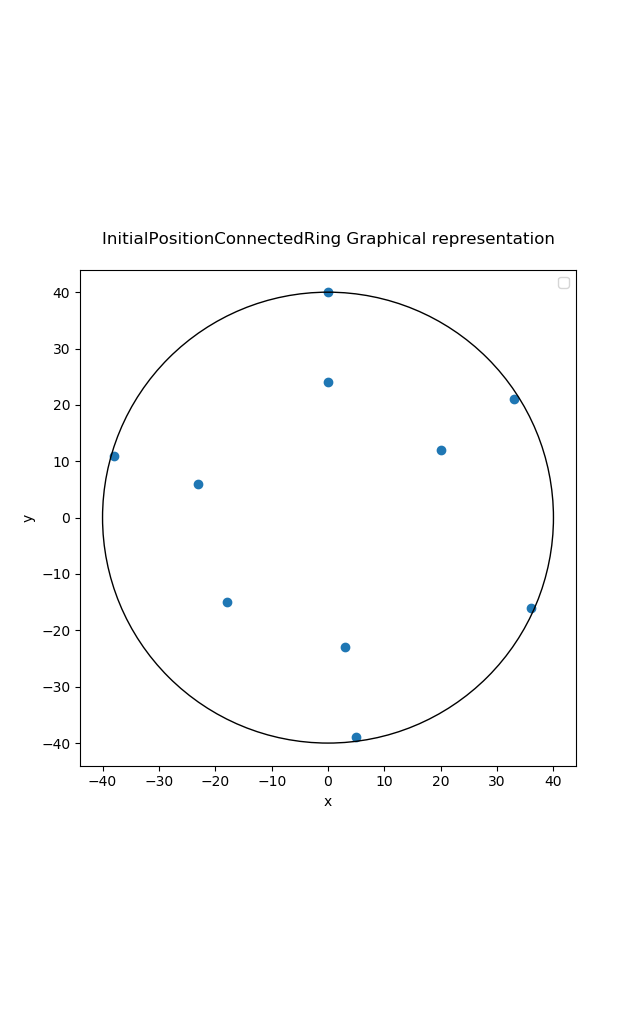
\includegraphics[width=0.5\textwidth, frame]{InitialPositionConnectedRing}
		\caption{Representation du placement InitialPotisionConnectedRing}
		\floatfoot{Le cercle represente le rayon (scope) et on voit bien que tous les nodes sont places autour d'un centre en (0,0). Pour se faire nous avons choisi une position initial (0,0). Cette position initiale est necessaire lors de l'appelle a la fonction \texttt{getNewPositionWith} qui fait partie de la classe Position}
		\label{fig:mesh1}
	\end{figure}



	\subsection*{Strategie 4 : InitialPositionConnectedRing (InitialPositionStrategy)}
	\subsubsection{\texttt{getInitialPosition}}
	Le but de cette strategie est de definir une position initiale pour tous les noeuds en une passe. C'est un chainage entre les noeuds vont se placer en fonction d'un voisin. Il existe un traitement specifique pour le tout premier noeud. L'algorithme redefini des bornes pour positionner le premier noeud. appelons les valeurs definies par defaut \texttt{old\_maxX} et \texttt{old\_maxY}. Cette nouvelle position est ajoutee a une \texttt{hashmap<id, Position>} qui s'appelle \texttt{initial\_position} qui est partagee par toutes les instances de cette classe.
	\begin{gather}
		Soit \quad (old\_maxX,old\_maxY) \in Entier^2 \\
		Soit \quad (minX,maxX,minY,maxY) \in Entier^4 \\
		Soit \quad p \in Position
		minX = old\_maxX / 3; \quad maxX = old\_maxX; \\
		minY = old\_maxY / 3; \quadmaxY = old\_maxY;\\
		p = ([minX, maxX], [minY, maxY]) \\
	\end{gather}
	Pour tous les autres noeuds,  ils choisissent un voisin qui possede un id egale a la taille de la hashmap \texttt{initial\_position}. ils choisissent au hasard, un angle, une distance bornee avec une verification que ces bornes sont bien definies grace a une fonction \texttt{bound}.
	Pour finir ils s'ajoutent a  la hashmap partagee.


	\subsection*{Stragerie 5 : NextDestinationConnectedOneMove (NextDestinationStrategy)}
	\subsubsection{\texttt{getNewPositionWith}}
	Le but de cette strategie est de definir une nouvelle position pour un node nomme \texttt{host} tout en gardant une seule composante connexe sur le reseau. Toute division en plusieurs composantes apres deplacement d'un noeud n'est pas retenu et le noeud reste immobile jusqu'a son prochain deplacement.
	\par Elle defini une variable qui represente le protocol du noeud \texttt{host} concerne par le deplacement appelee \texttt{pos\_proto\_host}
	\par Elle defini mais n'utilise pas un set qui associe a un \texttt{ID} de node une liste de noeuds qui est la composante connexe de ce noeud nommee \texttt{initial\_connected\_component}. Ce set est initialise par la ligne commande :
	\begin{lstlisting}[language=java]
		PositionProtocol.getConnectedComponents(PositionProtocol.getPositions(position_pid), scope);
	\end{lstlisting}
	\texttt{getConnectedComponents} : "méthode statique renvoyant l'ensemble des composantes connexes du système, renvoie une map associant un id de la composante connexe à son ensemble de noeud"
	\texttt{PositionProtocol.getPositions} : "méthodes statiques utiles pour toutes informations relative à la position des noeuds et à la topographie du système"
	\par Cette algorithme a aussi besoin du \texttt{scope} et defini un node \texttt{current\_moving} qui est le noeud precedemment mis en mouvement par l'appelle precedent de la fonction \texttt{getNewPositionWith}.
	\par \texttt{1ER PARTIE DE L'ALGO :}
	Le but est de stoper le noeud host s'il est en mouvement. Si le noeud \texttt{current\_moving} existe, alors il est stoppe et la fonction renvoie la valeur la position actuelle du noeud host.  Si le noeud ne bouge pas alors \textt{current\_moving} est remis a \texttt{null}.
	\par \texttt{2ND PARTIE DE L'ALGO :}
	Le noeud host n'est pas en mouvement et est autorise a bouger alors il choisi un voisin au hasard. un angle et une distance bornee par les bornes suivantes :
	\begin{gather}
		Soit \quad (distance\_min, distance\_max) \in ParametresDeBase \\
		min\_distance = min(scope, max(distance\_min, 0)) \\
		max\_distance = min(distance\_max, scope)
	\end{gather}

	La nouvelle position est cree et on verifie ses bornes. On recupere localement la liste desPositions des noeuds du reseau et on verifie s'il y a une division dans le reseau apres mise a jour de la position du node (un split qui serait du au deplacement du noeud sur sa nouvelle position). Si ce n'est pas le cas il devient le noeud \texttt{current\_moving} et renvoie la nouvelle position. Sinon il reste sur place. 




	\subsection*{Strategie 6 : NextDestinationImmobility (NextDestinationStrategy)}
	\subsubsection{\texttt{getNewPositionWith}}
	Cette strategie renvoie comme nouvelle position pour le node \texttt{host} la position actuelle du node host, il ne bouge pas.



	\subsection*{Strategie 7 : NextDestinationRandomPeriodicInitial (NextDestinationStrategy)}
	\subsubsection{\texttt{getNewPositionWith}}
	Cette strategie est parametre par une periode a specifier dans le fichier de configuration appelee \texttt{random\_dest\_period}. C'est une strategie possedant deux etats. Soit les noeuds sont a la position initiale, soit les noeuds appliquent la strategie FullRandom avec un placement completement aleatoire. Les noeuds sont places de maniere aleatoire pendant \texttt{random\_dest\_period} cycles de simulation. Ensuite ils passent tous en position initiale et retourne en positionnement aleatoire lorsque tous les noeuds sont passes dans l'etat initial.


	\newpage
	\chapter{Exercice 2 – Implémentation d’algorithmes d’élection de Leader sur un MANET}
	\section*{Premier algorithme}

	\begin{comment}
	an undirected graph that changes over time as nodes move. The vertices in the graph correspond to mobile nodes and an edge between a pair of nodes represents the fact that the two nodes are within each other’s transmission radii and, hence, can directly communicate with one another. The graph can become disconnected if the network is partitioned due to node movement
	\end{comment}



	\section{Question 1}
	\textit{Dans la section III, expliquez pour chaque hypothèse, pourquoi elle est vérifiée (ou peut être vérifiée) dans notre simulateur.}

	\subsection{Node Value:}
	\textit{"Each node has a value associated with it. The value of a node indicates its “desirability” as a leader of the network and can be any performance-related attribute such as the node’s battery power, computational capabilities etc."}

	l'interface ElectionProtocol est obligatoire pour implementer un protocol d'election. On peut voir y trouver une fonction avec le description suivante :
	\mylisting[basicstyle=\tiny,frame=rlbt,language=Java, firstline=17, lastline=21]{../src/ara/manet/algorithm/election/ElectionProtocol.java}


	\subsection{Unique and Ordered Node IDs:}
	\textit{"All nodes have unique identifiers. They are used to identify participants during the election process. Node IDs are used to break ties among nodes which have the same value."}

	Soit un node host, host.getID() a pour definition :
	\begin{lstlisting}[language=java]
	Returns the unique ID of the node. It is guaranteed that the ID is unique during the entire simulation, that is, there will be no different Node objects with the same ID in the system during one invocation of the JVM. Preferably nodes should implement hashCode() based on this ID.
	\end{lstlisting}

	\subsection{Links:}
	\textit{"Links are bidirectional and FIFO, i.e. messages are delivered in order over a link between two neighbors."}
	%TODO pas trouve

	\subsection{Node Behavior:}
	\textit{"Node mobility may result in arbitrary topology changes including network partitioning and merging. Furthermore, nodes can crash arbitrarily at any time and can come back up again at any time."}
	Cette propriete correspond aux differentes strategies de noeuds que nous avons decrite. Par exemple la strategie FullRandom peut autoriser des partitionnement ou des fusions.
	%TODO crash? did not implemented that 

	\subsection{Buffer Size:}
	\textit{"A message delivery is guaranteed only when the sender and the receiver remain connected (not partitioned) for the entire duration of message transfer."}

	Dans la classe EmitterProtocolImpl on peut voir la fonction recvMsg :
	\mylisting[basicstyle=\tiny,frame=rlbt,language=Java, firstline=44, lastline=66]{../src/ara/manet/communication/EmitterProtocolImpl.java}

	On peut voir dans cette fonction qu'on verifie bien ligne 19 que le la distance entre les noeuds est bien inferieur ou egale a la taille du scope qui permet la communication entre deux noeuds.

	\subsection{Node-to-Node Communications:}
	\textit{"Each node has a sufficiently large receive buffer to avoid buffer overflow at any point in its lifetime."}
	% TODO aucune idee mais je ne vois pas de limite dans notre programme

	\section{Question 2}

	\section{Question 3}

	\section{Question 4}

	\section*{Deuxieme algorithme}

	\section{Question 5}
	\textit{L’algorithme utilise des horloges logiques. A quoi servent-elles ?  Pourquoi chaque nœud ne peut incrémenter uniquement sa propre horloge ?}
	\section{Question 6}
	\textit{Pourquoi le knowledge est émis dans sa totalité à la détection de l’arrivée d’un nœud dans le voisinage ?}
	\section{Question 7}
	\textit{Quel est l’intérêt de créer des edits lors de la déconnexion d’un voisin ou de la réception d’un knowledge, au lieu d’envoyer le knowledge dans son ensemble ?}
	\section{Question 8}
	\textit{Quel est le contenu d’un edit ?}
	\section{Question 9}
	\textit{Qu’implique l’adjectif reachable ligne 46 ?}
	\section{Question 10}
	\textit{Implémentez l’algorithme dans PeerSim et vérifiez qu’il fonctionne avec le moniteur graphique.}
	\section{Question 11}
	\textit{Considérons maintenant qu’il puisse y avoir des pertes de messages suite aux collisions des ondes radio (on ne vous demande pas de les implémenter).}
	\begin{itemize}
		\item \textit{Quel impact ceci aurait sur les valeurs des horloges (old\_clock et knowledge[source].clock) lors des réceptions de edit ?}
		\item \textit{Comment pourrions-nous résoudre efficacement ce problème (encore une fois , il n’est pas demandé de l’implémenter)}
	\end{itemize}

	\newpage
	\chapter{Exercice 3 – Étude expérimentale}

	\newpage
	\bibliographystyle{IEEEtran}
	\bibliography{biblio}

	\newpage
	% \phantomsection
	\addcontentsline{toc}{chapter}{\listfigurename}
	\listoffigures



	\newpage
	\chapter{Annexe}




\end{document}

